\chapter{Utilities} \label{chap:Utils}

All utilities have command line help with short description when
\texttt{-h} argument is used. Besides \texttt{-h}, most of the utilities
have several standard command line options that are the same. The standard
options can be used with any utility unless stated otherwise.

\vspace{1em}
\noindent
\begin{tabular}{p{0.14\textwidth}p{0.804\textwidth}}
  \toprule
  \multicolumn{2}{l}{Standard options} \\
  \midrule
  \texttt{-i <name>} & use custom structure file instead of
    \texttt{traject.vsf} (it can also be a \texttt{vtf} file) \\
  \texttt{-v}        & verbose output that provides information about all
    bead and molecule types \\
  \texttt{-s}        & run silently, i.e., without any output at all
    (overrides \texttt{-v} option) \\
  \texttt{--script}  & no progress output (useful if output is routed to a
    file) \\
  \texttt{-h}        & print this help and exit \\
  \bottomrule
\end{tabular}

\section{AddToSystem} \label{sec:AddToSystem}

This utility takes an existing system specified by \texttt{vcf} coordinate
and \texttt{vsf} structure files and adds new beads into it. The new beads
replace neutral unbonded ones with the lowest indices (as ordered in the
\texttt{vsf} file) from the original system. If molecules are added,
\texttt{AddToSystem} places them at the end (for the sake of
\texttt{DL\_MESO} which requires molecules to be after unbonded beads). The
utility generates \texttt{vcf} and \texttt{vsf} files for the new system.

\texttt{AddToSystem} does not check whether there are enough unbonded
neutral beads to be replaced by the new beads.

The coordinates of the new unbonded beads are ruled by the \texttt{-ld},
\texttt{-hd}, and \texttt{-bt} options; the first bead of the new molecules
obey these options. The coordinates of the remaining beads in a molecule
are governed by the provided coordinates. The molecules are added with a
random orientation.

If \texttt{-ld} and/or \texttt{-hd} options are used, they must accompanied
by the \texttt{-bt} option.

The structure and number of added molecules and monomeric beads are read
from a \texttt{FIELD}-like file. This file must contain \texttt{species}
section followed by \texttt{molecule} section as described in the DL\_MESO
simulation package.

The \texttt{species} section contains the number of bead types and their
properties:
\begin{verbatim}
  species <int>
  <name>  <mass> <charge> <number of unbonded beads>
\end{verbatim}
The first line must start with \texttt{species} keyword followed by the
number of bead types. For each bead type a single line must contain the name of
the bead, their mass and charge, and a number of these beads that are not
in a molecule (i.e., monomeric beads).

The \texttt{molecule} section that must be behind the \texttt{species}
section contains information about structure and numbers of molecules to be
added:

\noindent
\begin{longtable}{ll}
  \texttt{molecule <int>} & number of types of molecules \\
  \texttt{<name>} & name of the first molecule type \\
  \texttt{nummols <int>} & number of these molecules \\
  \texttt{beads <int>} & number of beads in these molecules \\
  \texttt{<bead name> <float> <float> <float>} & a line for each of the \texttt{<int>} beads \\
  \texttt{...} & \ \ \ \ specifying bead name and \\
  \texttt{<bead name> <float> <float> <float>} & \ \ \ \ Cartesian coordinates \\
  \texttt{bonds <int>} & number of bonds in these molecule \\
  \texttt{<string> <int> <int>} & a line for each of the \texttt{<int>} bonds \\
  \texttt{...} & \ \ \ \ containing arbitrary string and \\
  \texttt{<string> <int> <int>} & \ \ \ \ indices connected beads \\
  \texttt{...} & anything beyond here is ignored \\
  \texttt{finish} & description of a molecule is finished \\
\end{longtable}

The \texttt{molecule} keyword specifies the number of molecule types, that
is the number of \texttt{finish} keywords that must be present. The
\texttt{<bead name>} must be present in the \texttt{species} section. The
arbitrary \texttt{<string>} in the \texttt{bonds} is ignored by
\texttt{AddToSystem} (it is a relic from the \texttt{DL\_MESO} simulation
package, where the \texttt{<string>} specifies a type of bond). The indices
in \texttt{bond} lines run from 1 to the number of beads in the molecules and are
ordered according to the \texttt{beads} part of the section. Because
\texttt{molecule} section in the \texttt{FIELD} file from \texttt{DL\_MESO}
can also include bond angles and dihedral angles, anything beyond the last
bond line is ignored (until the \texttt{finish} keyword is read).

If no molecules are to be added, the line \texttt{molecule 0} must be still
be present in the file.

The following is an example of the \texttt{FIELD}-like file:
\begin{verbatim}
  species 3
  A   1.0  1.0  0
  B   1.0  0.0  0
  CI  1.0 -1.0 30

  molecule 2
  Dimer
  nummols 10
  beads 2
  A 0.0 0.0 0.0
  A 0.5 0.0 0.0
  bonds 1
  harm 1 2
  finish
  surfact
  nummols 10
  beads 3
  A 0.0 0.0 0.0
  B 0.5 0.0 0.0
  B 1.0 0.0 0.0
  bonds 2
  harm 1 2
  harm 2 3
  angles 1
  harm 1 2 3
  finish
\end{verbatim}
In this example, 30 unbonded (or monomeric) negatively charged beads called
\texttt{CI} are added as well as 20 molecules -- 10 molecules called
\texttt{Dimer} and 10 molecules called \texttt{surfact}. \texttt{Dimer}
molecules contain two \texttt{A} beads and one bond each; \texttt{surfact}
molecules contain three beads and two bonds each. The part starting with
\texttt{angles} and ending with \texttt{finish} is ignored. All in all, 80
beads are added -- 30 \texttt{CI}, 30 \texttt{A}, and 20 \texttt{B} beads.

The utility creates the \texttt{vcf} and \texttt{vsf} files with the new
system and can also write the coordinates into a \texttt{xyz} file.

Usage:

\vspace{1em}
\noindent
\texttt{AddToSystem <input.vcf> <input add> <out.vcf> <out.vsf> <options>}

\vspace{1em}
\noindent
\begin{longtable}{p{0.235\textwidth}p{0.709\textwidth}}
  \toprule
  \multicolumn{2}{l}{Mandatory arguments} \\
  \midrule
  \texttt{<input>} & input coordinate file (either \texttt{vcf} or
    \texttt{vtf} format) \\
  \texttt{<input add>} & FIELD-like file specifying additions to the system \\
  \texttt{<out.vcf>} & output \texttt{vcf} coordinate file for the new
  system \\
  \texttt{<out.vsf>} & output \texttt{vsf} structure file for the new system \\
  \toprule
  \multicolumn{2}{l}{Non-standard options} \\
  \midrule
  \texttt{-st <int>} & timestep to add new beads to (default: 1) \\
  \texttt{-xyz <name>} & save coordinates to \texttt{xyz} file \\
  \texttt{-ld <float>} & lowest distance from beads specified by
    \texttt{-bt} option \\
  \texttt{-hd <float>} & highest distance from beads specified by
    \texttt{-bt} option \\
  \texttt{-bt <bead names>} & bead types to use in conjunction with
    \texttt{-ld} and/or \texttt{-hd} options \\
  \bottomrule
\end{longtable}

\section{Aggregates and Aggregates-NotSameBeads} \label{sec:Aggregates}

These utilities determine which molecules belong to which aggregates
according to a simple criterion: two molecules belong to the same aggregate
if they share at least a specified number of contact pairs. A contact pair
is a pair of two beads belonging to different molecules which are closer
than a specified distance. The information is written in \texttt{agg}
format described in Section~\ref{sec:AggFile}.

The number of contact pairs, the distance, and bead type(s) to use for
aggregate determination are all arguments of the utilities.  Any molecule
type(s) can be excluded from aggregate determination (\texttt{-x <mol
name(s)>} option); they are also excluded from the output \texttt{agg}
file).  Moreover, any molecules close to specified molecule(s) can be
excluded (\texttt{-xm <mol name(s)>} option); here, `close' means any of
the bead types used aggregate determination is closer than
\texttt{<distance>} to any bead of the specified molecule.

Also, periodic boundary conditions can be removed from whole aggregates and
the new coordinates saved to an indexed \texttt{vcf} file (\texttt{-j}
option). Therefore aggregates will not be split by simulation box
boundaries when, for example, visualizing the molecules with vmd.

While the \texttt{Aggregates} utility uses all possible pairs of given bead
types, \texttt{Aggrega}-\texttt{tes-NotSameBeads} does not use same-type pairs. For
example, if bead types \texttt{A} and \texttt{B} are given,
\texttt{Aggregates} will use all three possible bead type pairs (i.e.,
\texttt{A-A}, \texttt{A-B}, and \texttt{B-B}), but
\texttt{Aggregates-NotSameBeads} will use only \texttt{A-B} bead type
pairs.

Usage:

\noindent
\vspace{1em}
\texttt{Aggregates} (or \texttt{Aggregates-NotSameBeads}) \texttt{<input>
<distance> <contacts> <output.agg> <bead type name(s)> <options>}

\vspace{1em}
\noindent
\begin{longtable}{p{0.25\textwidth}p{0.694\textwidth}}
  \toprule
  \multicolumn{2}{l}{Mandatory arguments} \\
  \midrule
  \texttt{<input>} & input coordinate file (either \texttt{vcf} or
    \texttt{vtf} format) \\
  \texttt{<distance>} & minimum distance for two beads to be in contact
    (thus constituting a contact pair) \\
  \texttt{<contacts>} & minimum number of contact pairs between two
    molecules to be in one aggregate \\
  \texttt{<output.agg>} & output \texttt{agg} file (must end in
    \texttt{.agg}) with aggregate information \\
  \texttt{<bead type(s)>} & bead type name(s) to use for determining
    contact pairs (at least two for \texttt{Aggregates-NotSameBeads}) \\
  \texttt{<options>} & \\
  \toprule
  \multicolumn{2}{l}{Non-standard options} \\
  \midrule
  \texttt{-x <mol name(s)>} & exclude specified molecule type(s) from
    aggregate determination (and from the output \texttt{agg} file) \\
  \texttt{-xm <mol name(s)>} & exclude molecules that are close to
    specified molecule(s) \\
  \texttt{-j <output.vcf>} & output \texttt{vcf} file with coordinates of
    joined aggregates (i.e., without periodic boundary conditions) \\
  \bottomrule
\end{longtable}

\section{AngleMolecules} \label{sec:AngleMolecules}

This utility calculates angles between beads in each molecule of specified
molecule type(s). The beads do not have to be connected, so the angle does
not have to be between two bonds.

Using \texttt{-n} option, the angle is specified by three bead indices taken
from the order of beads in the \texttt{vsf} file. These indices go from 1
to $N$, where $N$ is the number of beads in the molecule type. Generally,
the numbering of beads inside a molecule is made according to the first
molecule of the given type in \texttt{vsf} file. For example, assume that
beads of the first molecule called \texttt{mol} in the \texttt{vsf} file
are ordered \texttt{A} (\texttt{vsf} index 123), \texttt{B} (\texttt{vsf}
index 124), \texttt{C} (\texttt{vsf} index 200). Then, bead \texttt{A} is
1, bead \texttt{B} is 2, and \texttt{C} is 3.

More than one angle can be specified (i.e., a multiple of three numbers
have to be supplied to the \texttt{-n} option.). For example, assuming
indices \texttt{1 2 3 1 3 2} are specified, two angles will be calculeted.
The first angle will be between lines defined by beads with indices
\texttt{1 2} and \texttt{2 3}; the second one will be between lines defined
by beads with indices \texttt{1 3} and \texttt{3 2}. An angle is calculated in
degrees and is between 0 and 180$^{\circ}$.

The utility calculates distribution of angles for each specified trio of
bead indices for each molecule type and prints overall averages at the end
of an \texttt{<output>} file. If \texttt{-a} option is used, it can also write
all the angles for all individual molecules in each timestep (i.e., time
evolution of the angle for each individual molecule).

Usage:

\vspace{1em}
\noindent
\texttt{AngleMolecules <input> <width> <output> <mol name(s)> <options>}

\noindent
\begin{longtable}{p{0.19\textwidth}p{0.754\textwidth}}
  \toprule
  \multicolumn{2}{l}{Mandatory arguments} \\
  \midrule
  \texttt{<input>} & input coordinate file (either \texttt{vcf} or
    \texttt{vtf} format) \\
  \texttt{<width>} & width of each bin of the distribution \\
  \texttt{<mol name(s)>} & molecule name(s) to calculcate angles for \\
  \texttt{<output>} & output file for distribution \\
  \toprule
  \multicolumn{2}{l}{Non-standard options} \\
  \midrule
  \texttt{--joined} & specify that \texttt{<input>} contains joined
    coordinates (i.e., periodic boundary conditions for molecules do not
    have to be removed) \\
  \texttt{-a <name>} & write all angles for all molecules in all timesteps
    to \texttt{<name>} \\
  \texttt{-n  <ints>} & multiple of three indices for angle calculation (default: 1 2 3) \\
  \texttt{-st <int>} & starting timestep for calculation (default: 1) \\
  \texttt{-e <int>} & ending timestep for calculation (default: none) \\
  \bottomrule
\end{longtable}

\noindent
Format of output files:
\begin{enumerate}[nosep,leftmargin=20pt]
  \item \texttt{<output>} -- distribution of angles
    \begin{itemize}[nosep,leftmargin=5pt]
      \item first line: command used to generate the file
      \item second line: angle-specifying bead indices (the dash-separated
        numbers correspond to indices inside every molecule and are the
        same as the arguments to the \texttt{-n} option) with the numbers
        in brackets corresponding to $n$th column of data for each molecule
        type
      \item third line: numbering of columns (i.e., column headers)
        \begin{itemize}[nosep,leftmargin=10pt]
          \item first is the centre of each bin in angles (governed by
            \texttt{<width>}); i.e., if \texttt{<width>} is 5$^{\circ}$,
            then the centre of bin 0 to 5$^{\circ}$ is 2.5, centre of bin 5
            to 10$^{\circ}$ is 7.5 and so on
          \item the rest are for the calculated data: the range for each
            molecule type specifies which column numbers correspond to the
            calculated angles for that particular molecule type and the
            order of angles is given by the second line
        \end{itemize}
      \item last two lines: arithmetic means for each calculated angle
        (last line) and headers (second to last line) that again give range
        of columns in the last line for each molecule type
    \end{itemize}
  \item \texttt{-a <name>} -- all angles for all molecules in all timesteps
  \begin{itemize}[nosep,leftmargin=5pt]
    \item first and second lines are the same as for \texttt{<output>}
    \item third line: column headers
      \begin{itemize}[nosep,leftmargin=10pt]
        \item first is simulation timestep
        \item the rest are the calculated data: the range for each molecule
          type corresponds to the number of molecules of the given type
          times the number of calculated angles; for each molecule the
          angles are ordered according to the second line
      \end{itemize}
  \end{itemize}
\end{enumerate}

\section{Average} \label{sec:Average}

This utility calculates one of three types of averages based on a used option
from specified column(s) of data in the input text file (all \tt{\#}-starting
lines and blank lines are ignored). It either produces an overall average with
statistical error and an autocorrelation time estimate (\tt{-tau} option),
block averages (\tt{-b} option), or moving averages (\tt{-m} option). While the
\tt{-tau} option appends a single line to the output file, either of the
\tt{-b} or \tt{-m} options creates a new output file with somewhat smoother
data.

The first and last lines used for the average calculation can be controlled
using the standard \tt{-st} and \tt{-e} options.

\subsection{Estimate autocorrelation time via -tau option}

The average value of an observable $\mathcal{O}$ is a simple arithmetic
mean,
\begin{equation} \label{eq:Average} %{{{
  \langle\mathcal{O}\rangle = \frac{1}{N} \sum^N_{i=1} \mathcal{O}_i,
\end{equation} %}}}
where $N$ is the number of measurements and the subscript $i$ denotes
individual measurements. If the measurements are independent (i.e.,
uncorrelated), the statistical error, $\epsilon$, is given by:
\begin{equation} \label{eq:IndependentError} %{{{
  \epsilon^2 =
    \frac{\sigma^2_{\mathcal{O}_i}}{N},
\end{equation} %}}}
where $\sigma^2_{\mathcal{O}_i}$
is the variance of the individual
measurements,
\begin{equation} %{{{
  \sigma^2_{\mathcal{O}_i} = \frac{1}{N-1} \sum^N_{i=1} (\mathcal{O}_i -
  \langle\mathcal{O}\rangle)^2.
\end{equation} %}}}

For correlated data, the autocorrelation time,
$\tau$, representing the number of steps between two uncorrelated
measurements must be determined. Every
$\tau$-th measurement is uncorrelated, so the
equation~\eqref{eq:IndependentError} can then be used to estimate the
error.

A commonly used method to estimate $\tau$
is the binning (or block) method. In this method, the correlated data are
divided into $N_{\mr{B}}$ non-overlapping blocks of size $k$ ($N=k
N_{\mr{B}}$) with per-block averages, $\mathcal{O}_{\mr{B},n}$,
defined as:
\begin{equation} \label{eq:BlockAverage} %{{{
  \mathcal{O}_{\mr{B},n} = \frac{1}{k}
    \sum^{k n}_{\substack{i=1+\\(n-1)k}} \mathcal{O}_i.
\end{equation} %}}}
If $k\gg\tau$, the blocks are assumed to be uncorrelated and
equation~\eqref{eq:IndependentError} can be used:
\begin{equation} \label{eq:Error} %{{{
  \epsilon^2 =
  \frac{\sigma^2_{\mr{B}} }{N_{\mr{B}} } = \frac{1}{N_{\mr{B}} (N_{\mr{B}}
  -1)} \sum^{N_{\mr{B}} }_{n=1} (\mathcal{O}_{\mr{B},n} -
  \overline{\mathcal{O}})^2.
\end{equation} %}}}
An estimate of the autocorrelation time can be obtained using the following
formula:
\begin{equation} \label{eq:tau} %{{{
  \tau_{\mathcal{O}} = \frac{k \sigma^2_{\mr{B}} }{2
  \sigma^2_{\mathcal{O}_i}}.
\end{equation} %}}}

The number of blocks, $N_{\mr{B}}$, is supplied as an argument of the \tt{-tau}
option and Average then appends a single line to the \tt{<output>} file; the
line starts with $N_{\mr{B}}$ and continues with three values
($\langle\mathcal{O}\rangle$, $\epsilon$, and $\tau_{\mathcal{O}}$) per every
data column specified in the Average command.

A way to quickly get a $\tau$ estimate is to use a wide range of $N_{\mr{B}}$
values and plot $\tau_{\mathcal{O}}$ from equation~\eqref{eq:tau} as a function
of $N_{\mr{B}}$. Because the number of data points in one block should be
significantly larger than the autocorrelation time (e.g., ten times larger),
plotting $f(x)=N/(10x)$ will produce a monotonously decreasing curve that
intersects the $\tau_{\mathcal{O}}$ vs. $N_{\mr{B}}$ curve. A value of
$\tau_{\mathcal{O}}$ near the intersection (but to the left, where the
decreasing curve is above $\tau_{\mathcal{O}}$ vs. $N_{\mr{B}}$ curve) can be
considered a safe estimate of $\tau$.

\subsection{Block averages via -b option}

Besides estimating the autocorrelation time, the per-block averages can be
themselves plotted to get (probably) smoother dataset. Using the \tt{-b} option,
the number of data points per block to average, $k$, is supplied, and the utility
prints the per-block averages from equation~\eqref{eq:BlockAverage} to the
output file.

This way of averaging could be useful for example with density data produced by
DensityBox or related utilities; if the bin width supplied to the DensityBox was
too small, it is (possibly much) faster to block-average the densities rather
than rerun DensityBox. For this case, specify the first column (distance) along
with any density columns from the density file.

\subsection{Moving averages via -m option}

More common way to smoothing noisy data is to use the moving (or rolling or
running) average (or moving mean or rolling mean); this common method does have
many names.

Similarly to the block-average, the first element of the moving average is a
simple mean of $k$ values. Unlike with block-average, however, the $k$ values
for the next element are obtained by ignoring only one value and taking the next
$k$ values; i.e., $k-1$ values from the previous element of the moving average
are always reused as opposed to the block-average where the blocks of data are
not overlapping.

The moving average elements, $\mathcal{O}_{\mr{M},n}$, are defined as
\begin{equation} \label{eq:MovingAverage}
  \mathcal{O}_{\mr{M},n} = \frac{1}{k}
    \sum^{n+k-1}_{n} \mathcal{O}_i.
\end{equation}

\vspace{1em}
\noindent
Usage: \tt{Average <input> <output> <column(s)>  [options]}
\noindent
\begin{longtable}{p{0.15\textwidth}p{0.794\textwidth}}
  \toprule
  \multicolumn{2}{l}{Mandatory arguments} \\
  \midrule
  \tt{<input>}     & input text file\\
  \tt{<output>}    & output text file\\
  \tt{<column(s)>} & at least one column number from \tt{<input>}\\
  \midrule
  \midrule
  \multicolumn{2}{l}{Options}\\
  \midrule
  \tt{-tau <int>} & $\tau$ estimation where \tt{<int>} represents the number of
                    blocks $N_{\mr{B}}$ \\
  \tt{-b <int>}   & block-average printing mode where \tt{<int>} represents
                    the number of data points per one block, $k$
                    (equation~\eqref{eq:BlockAverage})\\
  \tt{-m <int>}   & moving average mode where \tt{<int>} represents the number
                    of data points per one moving block, $k$
                    (equation~\eqref{eq:MovingAverage})\\
  \midrule
  \multicolumn{2}{l}{Other options (see the beginning of 
                     Chapter~\ref{chap:Utils})}\\
  \midrule
  \multicolumn{2}{l}{\tt{-st},
                     \tt{-e},
                     \tt{--verbose},
                     \tt{--silent},
                     \tt{--help},
                     \tt{--version}}\\
  \bottomrule
\end{longtable}

\section{BondLength} \label{sec:BondLength}

This utility calculates a distribution of bond lengths in specified
molecule(s). For each of the specified molecule type(s),
\texttt{BondLength} calculates bond lengths between all different types of
connected bead pairs.

For example, assume two linear molecule types \texttt{Mol\_1} and
\texttt{Mol\_2} both composed of bead types \texttt{A} and \texttt{B}.
\texttt{Mol\_1} is connected like this: \texttt{A-A-B}; \texttt{Mol\_2}
like this: \texttt{A-B-B}. If both molecule types are used,
\texttt{BondLength} calculates for each molecule type distribution of
lengths for bonds \texttt{A-A}, \texttt{A-B}, and \texttt{B-B} (separate
for each molecule even though the molecules share the same bead types).

Furthermore, \texttt{BondLength} can also calculate distribution of
distances between specified beads in each of the specified molecules. The
\texttt{-d} option takes as arguments pairs of bead indices (according to
the order of beads in the molecule in \texttt{vsf} -- similarly to the
\texttt{-c} option in \texttt{DensityMolecules}, i.e.,
Section~\ref{sec:DensityMolecules}). More than one pair can be specified.
These indices are the same for all \texttt{<mol name(s)>}. If an index
higher than the number of beads in the molecule is provided, the utility
takes the last bead of the molecule (i.e., the highest index). For example,
using \texttt{-d file.txt 1 2 1 999} would write two distributions for each
\texttt{<mol name(s)>} into \texttt{<file.txt>}: distribution of distances
between the first and second beads in each \texttt{<mol name(s)>} and
between the first and last (or 999th bead).

Usage:

\vspace{1em}
\noindent
\texttt{BondLength <input> <width> <output> <mol name(s)> <options>}

\noindent
\begin{longtable}{p{0.22\textwidth}p{0.724\textwidth}}
  \toprule
  \multicolumn{2}{l}{Mandatory arguments} \\
  \midrule
  \texttt{<input>} & input coordinate file (either \texttt{vcf} or
    \texttt{vtf} format) \\
  \texttt{<width>} & width of each bin of the distribution \\
  \texttt{<output>} & output file with distribution of bond lengths \\
  \texttt{<mol name(s)>} & molecule name(s) to calculcate bond lengths for \\
  \toprule
  \multicolumn{2}{l}{Non-standard options} \\
  \midrule
  \texttt{-st <int>} & starting timestep for calculation (default: 1) \\
  \texttt{-d <out> <ints>} & write distribution of distances
    between specified beads in each specified molecule to \texttt{<out>}\\
  \bottomrule
\end{longtable}

\noindent
Format of output files:
\begin{enumerate}[nosep,leftmargin=20pt]
  \item \texttt{<output>} -- distribution of bond length between all bead
    pairs
    \begin{itemize}[nosep,leftmargin=5pt]
      \item first line: command used to generate the file
      \item second line: column headers
        \begin{itemize}[nosep,leftmargin=10pt]
          \item first is the centre of each bin (governed by
            \texttt{<width>}); i.e., if \texttt{<width>} is 0.1,
            then the centre of bin 0 to 0.1 is 0.05, centre of bin 0.1 to
            0.2 is 0.15, etc.
          \item the rest are for the calculated data: for each molecule type,
            there is a list of column numbers corresponding to all
            possible bead type pairs in the molecule; if no beads of the
            given types are connected, the data column contains \texttt{nan}
        \end{itemize}
    \end{itemize}
  \item \texttt{-d <output> <ints>} -- distribution of distances between
    specified beads
    \begin{itemize}[nosep,leftmargin=5pt]
      \item first line: command used to generate the file
      \item second line: column headers
        \begin{itemize}[nosep,leftmargin=10pt]
          \item first is again the centre of every bin
          \item the rest are for the calculated data: for each molecule type,
            there is a list of column numbers corresponding to the given
            pairs of bead indices in the molecule
        \end{itemize}
    \end{itemize}
\end{enumerate}

\section{Config} \label{sec:Config}

This utility creates DL\_MESO \texttt{CONFIG} file. It requires input
coordinate file with all beads; otherwise the utility will still run, but
will produce incomplete \texttt{CONFIG}.

Usage:

\vspace{1em}
\noindent
\texttt{Config <input.vcf> <options>}

\vspace{1em}

\noindent
\begin{tabular}{p{0.15\textwidth}p{0.794\textwidth}}
  \toprule
  \multicolumn{2}{l}{Mandatory argument} \\
  \midrule
  \texttt{<input>}  & input coordinate file (either \texttt{vcf} or
    \texttt{vtf} format)\\
  \toprule
  \multicolumn{2}{l}{Non-standard option} \\
  \midrule
  \texttt{-st <int>} & timestep for creating \texttt{CONFIG} file from
    (default: last step) \\
  \bottomrule
\end{tabular}

\vspace{1em}
There is also utility \texttt{Config\_from\_xyz} which takes a \texttt{xyz}
coordinate file and creates the DL\_MESO \texttt{CONFIG} file. Because
\texttt{xyz} file does not contain information about the simulation box,
the resulting \texttt{CONFIG} file must be modified manually --
\texttt{Config\_from\_xyz} prints \texttt{x}, \texttt{y}, and \texttt{z}
into the output file where box dimensions should be.

Usage:

\vspace{1em}
\noindent
\texttt{Config\_from\_xyz <input.xyz> <options>}

\vspace{1em}

\noindent
\begin{tabular}{p{0.15\textwidth}p{0.794\textwidth}}
  \toprule
  \multicolumn{2}{l}{Mandatory argument} \\
  \midrule
  \texttt{<input>}  & input \texttt{xyz} coordinate file \\
  \toprule
  \multicolumn{2}{l}{Non-standard option} \\
  \midrule
  \texttt{-st <int>} & timestep for creating \texttt{CONFIG} file from
    (default: last step) \\
  \bottomrule
\end{tabular}

\section{DensityAggregates} \label{sec:DensityAggregates}

This utility calculates radial density profiles (RDPs, or radial number
densities) for bead types in an aggregate with specified size (the number
of molecules or aggregation number, $A_{\mathrm{S}}$) from its centre of
mass.

RDP$_i(r)$ of bead type $i$, where $r$ is distance from an aggregate's
centre of mass, is the number of these beads in a spherical shell between
the distances $r$ and $r+\mathrm{d}r$ (in \texttt{DensityAggregates},
$\mathrm{d}r$ is the \texttt{<width>} argument) divided by the
volume of this shell.

Composition of an aggregate with given size (i.e., average numbers of
different types of molecules in that aggregate) is appended to the output
file.
%The distance written in the output file is always $r+0.5\mathrm{d}r$.
%Besides RDP, the output file also contains radial number profiles (i.e.,
%the number of beads in the spherical shell not divided by the shell's
%volume) and one-sigma errors for both RDP and radial number profiles. The
%output file also contains a header describing what is in each column.

Instead of `true' aggregate size, a number of molecules of specific type(s)
can be used (\texttt{-m} option). For example, an aggregate containg 1
\texttt{Mol\_A} molecule and 2 \texttt{Mol\_B} molecules (i.e., three
molecules in all) can be specified in several ways:
\begin{enumerate}[nosep]
  \item  with \texttt{<agg size(s)>} of 3;
  \item  with \texttt{<agg size(s)>} of 3 and \texttt{-m Mol\_A Mol\_B};
  \item  with \texttt{<agg size(s)>} of 1 and \texttt{-m Mol\_A}; or
  \item  with \texttt{<agg size(s)>} of 2 and \texttt{-m Mol\_B}.
\end{enumerate}

Care must be taken when different molecule types share the same bead type.
If one bead type is in more molecule types, the resulting density for that
bead type will be the sum of its densities from all molecule types it
appears in. The \texttt{-x} option can overcome this -- specific molecule
types can be excluded from density calculations, i.e., density of beads in
the excluded molecule types will not be calculated.  For example, assume
two molecule types -- \texttt{Mol\_1} and \texttt{Mol\_2}.  \texttt{Mol\_1}
contains bead types \texttt{A} and \texttt{B}; \texttt{Mol\_2} contains
bead types \texttt{A} and \texttt{C}.  Depending on whether and how the
\texttt{-x} option is used, the utility will calculate:
\begin{enumerate}[nosep]
  \item densities of \texttt{A}, \texttt{B}, and \texttt{C} beads (density of
    \texttt{A} beads is a sum from both molecules), if no \texttt{-x} is used;
  \item densities of only \texttt{A} and \texttt{B} beads (with \texttt{A}
    beads only from \texttt{Mol\_1}), if \texttt{-x Mol\_2} is used;
  \item densities of only \texttt{A} and \texttt{C} beads (with \texttt{A}
    beads only from \texttt{Mol\_2}), if \texttt{-x Mol\_1} is used; or
  \item no densities at all if \texttt{-x Mol\_1 Mol\_2} is used.
\end{enumerate}
Therefore, to be able to plot density of \texttt{A} beads from
\texttt{Mol\_1} and \texttt{Mol\_2} separately, (2) and (3) should be used
(i.e., \texttt{DensityAggregates} should be run twice).

Usage:

\vspace{1em}
\noindent
\texttt{DensityAggregates <input> <input.agg> <width> <output> <agg \\
size(s)> <options>}

\noindent
\begin{longtable}{p{0.24\textwidth}p{0.704\textwidth}}
  \toprule
  \multicolumn{2}{l}{Mandatory arguments} \\
  \midrule
  \texttt{<input>} & input coordinate file (either \texttt{vcf} or
    \texttt{vtf} format) \\
  \texttt{<input.agg>} & input \texttt{.agg} file \\
  \texttt{<width>} & width of each bin of the distribution \\
  \texttt{<output>} & output file(s) (one per aggregate size) with
    automatic \texttt{\#.rho} ending (\texttt{\#} is aggregate size) \\
  \texttt{<agg size(s)>} & aggregate size(s) (the number of molecules in an
    aggregate or the aggregation number, $A_{\mathrm{S}}$) to calculcate
    density for \\
  \toprule
  \multicolumn{2}{l}{Non-standard options} \\
  \midrule
  \texttt{--joined} & specify that \texttt{<input>} contains joined
    coordinates (i.e., periodic boundary conditions for aggregates do not
    have to be removed) \\
  \texttt{-n <int>} & number of bins to average to get smoother density
    (default: 1) \\
  \texttt{-st <int>} & starting timestep for calculation (default: 1) \\
  \texttt{-e <int>} & ending timestep for calculation (default: none) \\
  \texttt{-m <mol name(s)>} & instead of `true' aggregate size, use the number
    of specified molecule type(s) in an aggregate \\
  \texttt{-x <mol name(s)>} & exclude specified molecule type(s) (i.e., do
    not calculate density for beads in molecules \texttt{<mol name(s)>}) \\
  \bottomrule
\end{longtable}

\noindent
Format of output files:
\begin{enumerate}[nosep,leftmargin=20pt]
  \item \texttt{<output>\#.rho} -- bead densities for one aggregate size
    \begin{itemize}[nosep,leftmargin=5pt]
      \item first line: command used to generate the file
      \item second line: the order of data columns for each bead type --
        \texttt{rdp} is radial density profile, \texttt{rnp} radial number
        profile and \texttt{stderr} are one-$\sigma$ errors for \texttt{rdp}
        and \texttt{rnp}
      \item third line: column headers
        \begin{itemize}[nosep,leftmargin=10pt]
          \item first is the centre of each bin (governed by
            \texttt{<width>}); i.e., if \texttt{<width>} is 0.1,
            then the centre of bin 0 to 0.1 is 0.05, centre of bin 0.1 to
            0.2 is 0.15, etc.
          \item the rest are for the calculated data: each number specifies
            the first column with data for the given bead type (i.e.,
            \texttt{rdp} column)
          \item last line contains the total number of aggregates the
            density was calculated for
        \end{itemize}
      \item second to last line: column headers for average numbers of
        different molecules in the given aggregate
      \item last line: average numbers of the molecules
    \end{itemize}
\end{enumerate}

\section{DensityBox} \label{sec:DensityBox}

This utility calculates number density for all bead types in the specified
direction of the simulation box. The density is calculated from 0 to box
length in the given direction.

Usage:

\vspace{1em}
\noindent
\texttt{DensityBox <input> <width> <output> <axis> <options>}

\noindent
\begin{longtable}{p{0.15\textwidth}p{0.794\textwidth}}
  \toprule
  \multicolumn{2}{l}{Mandatory arguments} \\
  \midrule
  \texttt{<input>} & input coordinate file (either \texttt{vcf} or
    \texttt{vtf} format) \\
  \texttt{<width>} & width of each bin of the distribution \\
  \texttt{<output>} & output file with automatic \texttt{<axis>.rho} ending \\
  \texttt{<axis>} & direction in which to calculate density: \texttt{x},
    \texttt{y}, or \texttt{z} \\
  \toprule
  \multicolumn{2}{l}{Non-standard options} \\
  \midrule
  \texttt{-n <int>} & number of bins to average to get smoother density
    (default: 1) \\
  \texttt{-st <int>} & starting timestep for calculation (default: 1) \\
  \bottomrule
\end{longtable}

\noindent
Format of output files:
\begin{enumerate}[nosep,leftmargin=20pt]
  \item \texttt{<output>} -- bead densities
    \begin{itemize}[nosep,leftmargin=5pt]
      \item first line: command used to generate the file
      \item second line: column headers
        \begin{itemize}[nosep,leftmargin=5pt]
          \item first is the centre of each bin (governed by
            \texttt{<width>}); i.e., if \texttt{<width>} is 0.1,
            then the centre of bin 0 to 0.1 is 0.05, centre of bin 0.1 to
            0.2 is 0.15, etc.
          \item the rest are for the calculated data: each number
            corresponds to the density of the specified bead type
        \end{itemize}
    \end{itemize}
\end{enumerate}

\section{DensityMolecules} \label{sec:DensityMolecules}

This utility works similarly to \texttt{DensityAggregates}, only instead
for whole aggregates, RDPs are calculated for individual molecules.
Similarly to \texttt{DensityAggregates}, the output file(s) also contain
statistical errors and radial number profiles.

By default, the utility calculates RDPs from the molecule's centre of mass,
but any bead in the molecule (with an index according to \texttt{vsf} --
similarly to \texttt{-n} option in \texttt{AngleMolecules},
Section~\ref{sec:AngleMolecules}) can be used instead (\texttt{-c} option).

Usage:

\vspace{1em}
\noindent
\texttt{DensityMolecules <input> <width> <output> <mol name(s)> <options>}

\noindent
\begin{longtable}{p{0.22\textwidth}p{0.724\textwidth}}
  \toprule
  \multicolumn{2}{l}{Mandatory arguments} \\
  \midrule
  \texttt{<input>} & input coordinate file (either \texttt{vcf} or
    \texttt{vtf} format) \\
  \texttt{<width>} & width of each bin of the distribution \\
  \texttt{<output>} & output file with automatic \texttt{<mol\_name>.rho}
    ending (one file per molecule type is generated) \\
  \texttt{<mol name(s)>} & molecule name(s) to calculcate density for \\
  \toprule
  \multicolumn{2}{l}{Non-standard options} \\
  \midrule
  \texttt{--joined} & specify that \texttt{<input>} contains joined
    coordinates (i.e., periodic boundary conditions for molecules do not
    have to be removed) \\
  \texttt{-n <int>} & number of bins to average for smoother density
    (default: 1) \\
  \texttt{-st <int>} & starting timestep for calculation (default: 1) \\
  \texttt{-e <int>} & ending timestep for calculation (default: none) \\
  \texttt{-c <name> <int>} & use specified bead in a molecule
    \texttt{<name>} instead of its centre of mass \\
  \bottomrule
\end{longtable}

\noindent
Format of output files:
\begin{enumerate}[nosep,leftmargin=20pt]
  \item \texttt{<output><mol\_name>.rho} -- bead densities for one molecule
    \begin{itemize}[nosep,leftmargin=5pt]
      \item first line: command used to generate the file
      \item second line: the order of data columns for each bead type --
        \texttt{rdp} is radial density profile, \texttt{rnp} is radial number
        profile and \texttt{stderr} are one-$\sigma$ errors for \texttt{rdp}
        and \texttt{rnp}
      \item third line: column headers
        \begin{itemize}[nosep,leftmargin=10pt]
          \item first is the centre of each bin (governed by
            \texttt{<width>}); i.e., if \texttt{<width>} is 0.1,
            then the centre of bin 0 to 0.1 is 0.05, centre of bin 0.1 to
            0.2 is 0.15, etc.
          \item the rest are for the calculated data: each number specifies
            the first column with data for the given bead type (i.e.,
            \texttt{rdp} column)
        \end{itemize}
    \end{itemize}
\end{enumerate}

\section{DihedralMolecules} \label{sec:DihedralMolecules}

This utility calculates angles between specified planes in each molecule of
specified molecule type(s). The planes in a molecule are arbitrary, so they
can represent true dihedral angles or improper dihedrals.

The angle is specified by six bead indices (according to the order of beads
in the molecule in \texttt{vsf} -- similarly to the \texttt{-n} option in
\texttt{AngleMolecules}, Section~\ref{sec:AngleMolecules}). The
first three indices specify one plane and the next three the other. For
example, assuming indices \texttt{1 2 3 4 5 6}, the first plane is
specified by the first three beads in the molecule; second plane by the
next three beads (beads \texttt{4 5 6}). The default indices
(i.e., if \texttt{-n} option is not used) are \texttt{1 2 3 2 3 4}. More
than one angle can be specified (i.e., a multiple of six numbers have to be
supplied to the \texttt{-n} option.).

The utility calculates distribution of angles for each specified trio of
bead indices for each molecule type and prints overall averages at the end
of \texttt{<output>} file. If \texttt{-a} option is used, it can also write
all the angles for all individual molecules in each timestep (i.e., time
evolution of the angle for each individual molecule).

Usage:

\vspace{1em}
\noindent
\texttt{DihedralMolecules <input> <mol name(s)> <options>}

\noindent
\begin{longtable}{p{0.235\textwidth}p{0.709\textwidth}}
  \toprule
  \multicolumn{2}{l}{Mandatory arguments} \\
  \midrule
  \texttt{<input>} & input coordinate file (either \texttt{vcf} or
    \texttt{vtf} format) \\
  \texttt{<output>} & output file for distribution \\
  \texttt{<mol name(s)>} & molecule name(s) to calculcate angles for \\
  \toprule
  \multicolumn{2}{l}{Non-standard options} \\
  \midrule
  \texttt{--joined} & specify that \texttt{<input>} contains joined
    coordinates (i.e., periodic boundary conditions for molecules do not
    have to be removed) \\
  \texttt{-a <file>} & write all angles for all molecules in all timesteps
    to \texttt{<file>} \\
  \texttt{-n  <ints>} & multiple of six indices for angle calculation
    (default: 1 2 3 2 3 4) \\
  \texttt{-st <int>} & starting timestep for calculation (default: 1) \\
  \bottomrule
\end{longtable}

\noindent
Format of output files:
\begin{enumerate}[nosep,leftmargin=20pt]
  \item \texttt{<output>} -- distribution of angles
    \begin{itemize}[nosep,leftmargin=5pt]
      \item first line: command used to generate the file
      \item second line: calculated angles (the dash-separated numbers
        correspond to indices inside every molecule and are the same as the
        arguments to the \texttt{-n} option) with the numbers in brackets
        corresponding to $n$th column of data for each molecule type
      \item third line: numbering of columns (i.e., column headers)
        \begin{itemize}[nosep,leftmargin=10pt]
          \item first is the centre of each bin in angles (governed by
            \texttt{<width>}); i.e., if \texttt{<width>} is 5$^{\circ}$,
            then the centre of bin 0 to 5$^{\circ}$ is 2.5, centre of bin 5
            to 10$^{\circ}$ is 7.5 and so on
          \item the rest are for the calculated data: the range for each
            molecule type specifies which column numbers correspond to the
            calculated angles for that particular molecule type and the
            order of angles is given by the second line
        \end{itemize}
      \item last two lines: arithmetic means for each calculated angle
        (last line) and headers (second to last line) that again give range
        of columns in the last line for each molecule type
    \end{itemize}
  \item \texttt{-a <file>} -- all angles for all molecules in all timesteps
  \begin{itemize}[nosep,leftmargin=5pt]
    \item first and second lines are the same as for \texttt{<output>}
    \item third lines: column headers
      \begin{itemize}[nosep,leftmargin=10pt]
        \item first is simulation timestep
        \item the rest are the calculated data: the range for each molecule
          type corresponds to the number of molecules of the given type
          times the number of calculated angles; for each molecule the
          angles are ordered according to the second line
      \end{itemize}
  \end{itemize}
\end{enumerate}

\section{DistrAgg} \label{sec:DistrAgg}

This utility calculates average aggregate mass and aggregation number for
each timestep (i.e., time evolution) and the averages over all timesteps
from a supplied \texttt{agg} file (see Section~\ref{sec:AggFile} for its format).
It calculates number, weight, and z averages. It also calculates
distribution functions of aggregation sizes and volumes.

For a quantity $\mathcal{O}$, the number, weight, and z averages,
$\langle\mathcal{O}\rangle_{\mathrm{n}}$,
$\langle\mathcal{O}\rangle_{\mathrm{w}}$, and
$\langle\mathcal{O}\rangle_{\mathrm{z}}$, respectively, are defined as
\begin{equation} \label{eq:Avg}
  \langle\mathcal{O}\rangle_{\mathrm{n}} = \frac{\sum_i N_i\mathcal{O}_i     }{N}
  \mbox{, \ \ \ }
  \langle\mathcal{O}\rangle_{\mathrm{w}} = \frac{\sum_i N_im_i\mathcal{O}_i  }{\sum_i N_i m_i}
  \mbox{, and \ \ \ }
  \langle\mathcal{O}\rangle_{\mathrm{z}} = \frac{\sum_i N_im_i^2\mathcal{O}_i}{\sum_i N_i m_i^2},
\end{equation}
where $N$ is the total number of measurements, i.e., the total number of
aggregates for per-aggregate averages (or molecules for per-molecule
averages); $N_i$ is the number of measurements with the value
$\mathcal{O}_i$, and $m_i$ is mass of an aggregate $i$ (or a molecule $i$).

Per-timestep averages are written to the \texttt{<output avg>} and overall
averages are appended as comments (with commented legend) to both
\texttt{<output avg>} and \texttt{<output distr>} files.

Number, weight, and z distribution functions of aggregate sizes,
$F_{\mathrm{n}}(A_{\mathrm{S}})$, $F_{\mathrm{w}}(A_{\mathrm{S}})$, and
$F_{\mathrm{z}}(A_{\mathrm{S}})$ respectively, are defined as
\begin{equation} \label{eq:Fnwz}
  \arraycolsep=1.4pt\def\arraystretch{2.5}
  \begin{array}{>{\displaystyle}rc>{\displaystyle}l}
    F_{\mathrm{n}} & = & \frac{N_{A_{\mathrm{S}} }}{\sum_{A_{\mathrm{S}} } N_i} =
    \frac{N_{A_{\mathrm{S}} }}{N}
  \mbox{,} \\
    F_{\mathrm{w}} & = & \frac{N_{A_{\mathrm{S}} } m_{A_{\mathrm{S}} }}{\sum_{A_{\mathrm{S}} } N_i m_i} =
    \frac{N_{A_{\mathrm{S}} } m_{A_{\mathrm{S}} }}{\sum_{i=1}^N m_i} =
    \frac{N_{A_{\mathrm{S}} } m_{A_{\mathrm{S}} }}{M}
  \mbox{, and} \\
    F_{\mathrm{z}} & = & \frac{N_{A_{\mathrm{S}} } m^2_{A_{\mathrm{S}}
    }}{\sum_{A_{\mathrm{S}} } N_i m_i^2} =
    \frac{N_{A_{\mathrm{S}} } m^2_{A_{\mathrm{S}} }}{\sum_{i=1}^N m_i^2}, \\
  \end{array}
\end{equation}
where $N_{A_{\mathrm{S}}}$ and $m_{A_{\mathrm{S}}}$ stand for the number
and mass, respectively, of aggregates with aggregate size $A_{\mathrm{S}}$;
$M$ is the total mass of all aggregates. The equations are normalised so
that $\sum F_x(A_{\mathrm{S}})=1$.

Distribution of volume fractions of aggregates, $\phi(A_{\mathrm{S}})$, is
defined (assuming all beads have the same volume) as

\begin{equation} \label{eq:Fvol}
  \phi(A_{\mathrm{S}}) = \frac{N_{A_{\mathrm{S}} } m_{A_{\mathrm{S}} }}{\sum_{i=1}^N n_i} =
  \frac{N_{A_{\mathrm{S}} } m_{A_{\mathrm{S}} }}{n},
\end{equation}
where $n_i$ is the number of beads in aggregate $i$ and $n$ is the total
number of beads in all aggregates. If all beads have unit mass (as is often
the case in dissipative particle dynamics), the volume distribution,
$\phi(A_{\mathrm{S}})$, is equal to the number distribution,
$F_{\mathrm{n}}(A_{\mathrm{S}})$.
All distributions are written into the \texttt{<output distr>} file.

Lastly, \texttt{DistrAgg} can calculate number distribution of composition
for aggregates with specified size(s) (\texttt{-c} option), that is, the
distribution of the numbers of different molecule types in the aggregate.
For example, if the simulation box contains molecule types \texttt{Mol\_A}
and \texttt{Mol\_B}, aggregates with the same size can contain different
numbers of these molecules, or different ratios of the numbers of
\texttt{Mol\_A} to \texttt{Mol\_B} molecules,
$\xi=N_{\mathrm{Mol\_A}}/N_{\mathrm{Mol\_B}}$. For now, \texttt{DistriAgg}
can calculate this distribution only for aggregates containing two molecule
types. The composition distribution is defined as
\begin{equation} \label{eq:CompDistr}
  F_{\mathrm{n}}(\xi) = \frac{N_{\xi,A_{\mathrm{S}} }}{N_{A_{\mathrm{S}}} },
\end{equation}
where $N_{\xi,A_{\mathrm{S}} }$ is the number of aggregates with aggregate
size $A_{\mathrm{S}}$ and ratio $\xi$; $N_{A_{\mathrm{S}}}$ is the total
number of aggregates with aggregate size $A_{\mathrm{S}}$.
\textit{Unfortunatly, this option may not work correctly.}

The definition of aggregate size is flexible. If none of \texttt{-m},
\texttt{-x}, or \texttt{--only} options is used, aggregate size is the
\say{true} aggregation number, $A_{\mathrm{S}}$, i.e., the number of all
molecules in the aggregate; if \texttt{-m} is used, aggregate size is the
sum of only specified molecule type(s); if \texttt{-x} is used, aggregates
containing only specified molecule type(s) are disregarded; if
\texttt{--only} is used, only aggregates composed of the specified molecule
type(s) are taken into account. For example, consider a system containing
three aggregates composed of various numbers of three different molecule
types:

\begin{longtable}{c|l}
  \toprule
  Molecule types & \multicolumn{1}{c}{Aggregate composition} \\
  \midrule
  \texttt{Mol\_A} & \texttt{Agg\_1}: 1 \texttt{Mol\_A} $+2$ \texttt{Mol\_B} $+3$ \texttt{Mol\_C} $=6$ molecules \\
  \texttt{Mol\_B} & \texttt{Agg\_2}: 1 \texttt{Mol\_A} $+2$ \texttt{Mol\_B} $=3$ molecules \\
  \texttt{Mol\_C} & \texttt{Agg\_3}: 1 \texttt{Mol\_A} $=1$ molecule \\
  \bottomrule
\end{longtable}

\noindent
Here is a list of some of the possibilities depending on the option(s)
used:
\begin{enumerate}[nosep]
  \item if none of \texttt{-m}, \texttt{-x}, \texttt{--only} is used, all
    three aggregates are counted and their sizes are their aggregation
    numbers, i.e., $A_{\mathrm{S}}=6$, 3, and 1
  \item if \texttt{-m Mol\_A Mol\_B} is used, all three aggregates are
    counted, but their size is the sum of only \texttt{Mol\_A} and
    \texttt{Mol\_B} molecules: \texttt{Agg\_1} -- 3; \texttt{Agg\_2} -- 3;
    \texttt{Agg\_3} -- 1
  \item if \texttt{-m Mol\_B Mol\_C} is used, \texttt{Agg\_3} is not
    counted, because its size would be zero; \texttt{DistrAgg} would detect
    only two aggregates with sizes: \texttt{Agg\_1} -- 5; \texttt{Agg\_2} --
    2
  \item if \texttt{-x Mol\_A Mol\_B} is used, \texttt{Agg\_2} and
    \texttt{Agg\_3} are not counted, because neither contains anything else
    than \texttt{Mol\_A} and/or \texttt{Mol\_B}; \texttt{DistrAgg} would
    detect only one aggregate with size: \texttt{Agg\_1} -- 6
  \item if \texttt{-x Mol\_A Mol\_B} is combined with \texttt{-m Mol\_A
    Mol\_B}, \texttt{DistrAgg} would again detect only \texttt{Agg\_1}, but
    its size would be 3
  \item if \texttt{--only Mol\_A Mol\_B} is used, \texttt{Agg\_1} is not
    counted, because it contains a molecule not specified by
    \texttt{--only}; \texttt{DistrAgg} would detect two aggregates
    with sizes: \texttt{Agg\_2} -- 3; \texttt{Agg\_3} -- 1
  \item if \texttt{--only Mol\_A Mol\_B} is combined with \texttt{-m
    Mol\_A}, the two detected aggregates have sizes: \texttt{Agg\_2} -- 1;
    \texttt{Agg\_3} -- 1
  \item if \texttt{--only Mol\_A Mol\_B} is combined with \texttt{-x
    Mol\_A}, only \texttt{Agg\_2} is detected as it is the only one composed of
    only \texttt{Mol\_A} and \texttt{Mol\_B} molecules and its size would
    be 3
  \item if \texttt{--only Mol\_A Mol\_B} and \texttt{-x Mol\_A} are combined
    with \texttt{-m Mol\_A}, the size of the aggregate would be 1
\end{enumerate}

Moreover, only a specified range of aggregate sizes can be taken into
account (\texttt{-n <int> <int>} option). These sizes are defined by the
\texttt{-m}, \texttt{-x}, and \texttt{--only} options as well.

Usage:

\vspace{1em}
\noindent
\texttt{DistrAgg <input.agg> <distr file> <avg file> <options>}

\noindent
\begin{longtable}{p{0.30\textwidth}p{0.644\textwidth}}
  \toprule
  \multicolumn{2}{l}{Mandatory arguments} \\
  \midrule
  \texttt{<input.agg>} & input \texttt{agg} file \\
  \texttt{<distr file>} & output file with distribution of aggregate
    sizes \\
  \texttt{<avg file>} & output file with per-timestep averages \\
  \toprule
  \multicolumn{2}{l}{Non-standard options} \\
  \midrule
  \texttt{-st <int>} & starting timestep for calculation (default: 1) \\
  \texttt{-n <int> <int>} & use aggregate sizes in a given range \\
  \texttt{-m <mol name(s)>} & use number of specified molecule(s) as
    aggregate size \\
  \texttt{-x <mol name(s)>} & exclude aggregates containing only specified
    mole\-cule(s) \\
  \texttt{--only <mol name(s)>} & use only aggregates composed of specified
    molecule(s) \\
  \texttt{-c <output> <int(s)>} & save composition distribution for
    specified aggregate size(s) to \texttt{<output>} file \\
  \bottomrule
\end{longtable}

\noindent
Format of output files:
\begin{enumerate}[nosep,leftmargin=20pt]
  \item \texttt{<output distr>} -- distributions of aggregate sizes
    \begin{itemize}[nosep,leftmargin=5pt]
      \item first line: command used to generate the file
      \item second line: column headers
        \begin{itemize}[nosep,leftmargin=10pt]
          \item first is the aggregate size, \texttt{As} -- either true aggregation
            number, or the size specified by options
          \item \texttt{F\_n(As)}, \texttt{F\_w(As)}, and \texttt{F\_z(As)} are
            number, weight, and z distribution of aggregate sizes (Equation
            \eqref{eq:Fnwz})
          \item \texttt{<volume distribution>} is distribution according
            to Equation \eqref{eq:Fvol}
          \item next is the total number of aggregates with specified size
          \item the remaining columns (\texttt{<mol name>\_n}) show average
            numbers of every molecule type in an aggregate with the
            specified size
        \end{itemize}
      \item second to last line: column headers for overall averages
        written in the last line
        \begin{itemize}[nosep,leftmargin=10pt]
          \item \texttt{<M>\_n}, \texttt{<M>\_w}, and \texttt{<M>\_z} are
            number, weight, and z averages, respectively, of aggregate
            masses (the averages are defined in Equation~\eqref{eq:Avg})
          \item other column headers are the same as at the file beginning
        \end{itemize}
    \end{itemize}
  \item \texttt{<output avg>} -- per-timestep averages
  \begin{itemize}[nosep,leftmargin=5pt]
    \item first line: command used to generate the file
    \item second lines: column headers
      \begin{itemize}[nosep,leftmargin=10pt]
        \item first is simulation timestep
        \item the rest are for the calculated data: number, weight, and z
          average aggregate mass (\texttt{<M>\_n}, \texttt{<M>\_w}, and
          \texttt{<M>\_z}, respectively) and aggregate size
          (\texttt{<As>\_n}, \texttt{<As>\_w}, and \texttt{<As>\_z},
          respectively) and the last column is the number of aggregates in
          the given step
      \end{itemize}
    \item the last two lines are the same as in \texttt{<output distr>}
  \end{itemize}
\item \texttt{-c <name>} -- composition distribution
  \begin{itemize}[nosep,leftmargin=5pt]
    \item first line: command used to generate the file
    \item second lines: column headers
      \begin{itemize}[nosep,leftmargin=10pt]
        \item first is ratio of the two molecule types (i.e., 0 to 1)
        \item the rest are aggregate sizes
        \item in the data, only ratios that are non-zero for at least one
          aggregate size are written; in case of more than one aggregate
          size specified by \texttt{-a} option, if the ratio does not exist
          for some aggregate size(s), `?' is displayed instead of zero
      \end{itemize}
  \end{itemize}
\end{enumerate}

\section{GenLayers} \label{sec:GenLayers}

This utility generates two monolayers composed of molecules specified in a
\texttt{FIELD}-like file. For now, only one type of molecule is used (the
first one in the \texttt{FIELD}-like file; other molecule types are
ignored). The two layers are mirror images of each other, that is,
molecules in both layers are grown from box edge to box middle (or the
first beads in the molecules are farthest from each other while the last
ones are closest to each other). The layers are placed in $z$ direction
(that is, in $xy$ planes of the simulation box).

The first beads of the molecules are arranged on a square lattice defined
either by given spacing in $x$ and $y$ directions (\texttt{-s} option) or
by the number of molecules per layer (\texttt{-nm} option). By default,
\texttt{GenLayers} places the two mirror layers at the edges of a
simulation box, but using the \texttt{-g} option, a gap from box edge can
be in introduced. Therefore, this utility can generate, for example,
polymer brushes at box edges or a double layer (such as a biological
membrane) in the middle of the box.

By default, the total number of beads in generated system is equal to three
times the box volume, that is, the typical number of beads in dissipative
particle dynamics simulations. Beads that are not in the molecules, are put
at the beginning of the output file with coordinates of the box centre and
name \texttt{None}. The idea is that once the layers are generated,
\texttt{AddToSystem} utility (see Section~\ref{sec:AddToSystem}) can be
used to exchange these excess beads for different species. The \texttt{-n}
option changes the total number of beads. If the number is lower than the
total number of beads needed to construct the two layers of molecules, it
is adjusted to exactly that number.

The input \texttt{FIELD}-like file must contain \texttt{species} and
\texttt{molecule} sections, but the \texttt{interaction} section is ignored
(see \texttt{DL\_MESO} manual for details on the \texttt{FIELD} file). The
first line of \texttt{FIELD} that is ignored by \texttt{DL\_MESO} must
start with box dimensions, i.e., with three numbers (the rest of the file
is ignored).

This utility does not have error checking for the provided
\texttt{FIELD}-like file. If the file is not correct, \texttt{GenLayers}
will exhibit undefined behaviour, that is, it will either freeze, crash, or
run without errors, producing bad output files.

The following snapshot is an example output using command \texttt{GenLayers
out.vsf out.vcf -n 1 -nm 50 -g 1} (the transparent squares are just a
visual aid) with the provided \texttt{FIELD}-like file:

\hfill
\begin{minipage}{0.4\textwidth}

  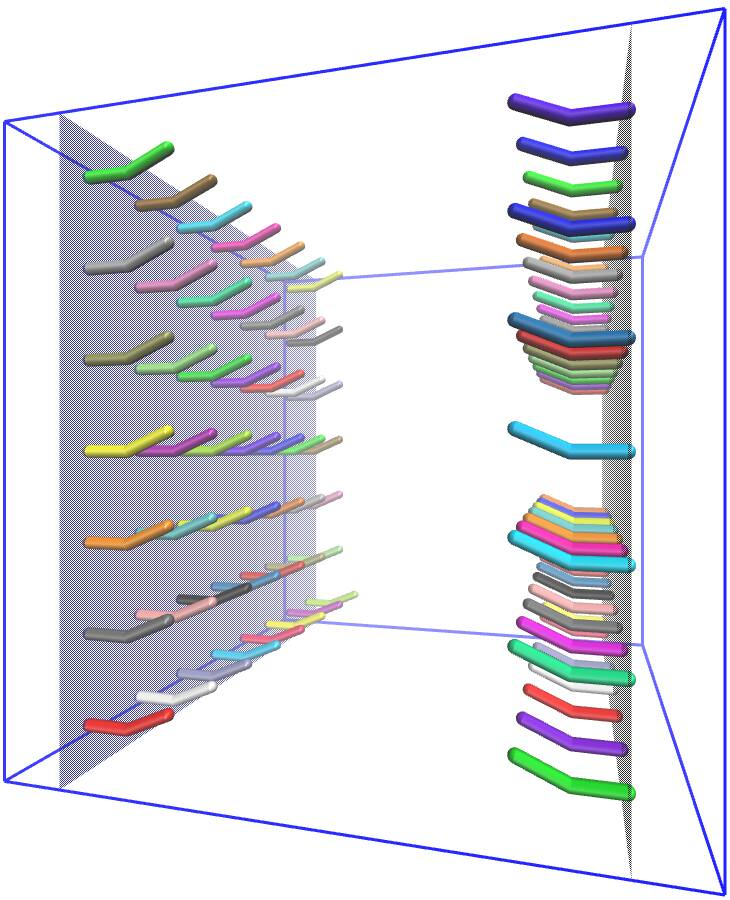
\includegraphics[width=\textwidth]{GenLayers-478ctac.jpg}
\end{minipage}
\begin{minipage}{0.5\textwidth}
  \centering
  \texttt{FIELD}
  \vspace{-1em}

\begin{verbatim}
   10 10 10
   species 1
   A   1.0 0.0 0
   molecules 1
   A3
   nummols 1
   beads 3
   A 0 0.0 0.0
   A 0 0.0 0.7
   A 0 0.3 1.4
   bonds 2
   harm 1 2 100.0 0.7
   harm 2 3 100.0 0.7
   finish
\end{verbatim}
\end{minipage}

The utility generates \texttt{vsf} structure and \texttt{vcf} coordinate
files.

Usage (\texttt{GenLayers} does not use standard options):

\vspace{1em}
\noindent
\texttt{GenSystem <out.vsf> <out.vcf> <options>}

\noindent
\begin{longtable}{p{0.15\textwidth}p{0.794\textwidth}}
  \toprule
  \multicolumn{2}{l}{Mandatory arguments} \\
  \midrule
  \texttt{<out.vsf>} & output \texttt{vsf} structure file \\
  \texttt{<out.vcf>} & output \texttt{vcf} coordinate file \\
  \toprule
  \multicolumn{2}{l}{Options} \\
  \midrule
  \texttt{-f <name>} & FIELD-like file (default: FIELD)\\
  \texttt{-v}        & verbose output that provides information about all
    bead and molecule types \\
  \texttt{-h}        & print help and exit \\
  \bottomrule
\end{longtable}

\section{GenSystem} \label{sec:GenSystem}

This simple utility uses modified \texttt{FIELD} file to create
\texttt{vsf} structure file and to generate coordinates that could be used
as a simulation's starting point. The utility assumes linear chains and
uses equilibrium bond length to construct a prototype molecule that is
fully stretched in one direction for each molecule type. The utility then
creates layers of molecules that are separated by layers of unbonded beads
(if there are any). The utility should fill the whole box with given beads.

The input \texttt{FIELD} file must contain \texttt{species} and
\texttt{molecule} sections, but the \texttt{interaction} section is ignored
(see \texttt{DL\_MESO} manual for details on the \texttt{FIELD} file). The
first line of \texttt{FIELD} that is ignored by \texttt{DL\_MESO} must
start with box dimensions, i.e., with three numbers (the rest of the file
is ignored).

Usage (\texttt{GenSystem} does not use standard options):

\vspace{1em}
\noindent
\texttt{GenSystem <out.vsf> <out.vcf> <options>}

\noindent
\begin{longtable}{p{0.15\textwidth}p{0.794\textwidth}}
  \toprule
  \multicolumn{2}{l}{Mandatory arguments} \\
  \midrule
  \texttt{<out.vsf>} & output \texttt{vsf} structure file \\
  \texttt{<out.vcf>} & output \texttt{vcf} coordinate file \\
  \toprule
  \multicolumn{2}{l}{Options} \\
  \midrule
  \texttt{-f <name>} & FIELD-like file (default: FIELD)\\
  \texttt{-v}        & verbose output that provides information about all
    bead and molecule types \\
  \texttt{-h}        & print help and exit \\
  \bottomrule
\end{longtable}

\section{GyrationAggregates} \label{sec:GyrationAggregates}

This utility calculates the gyration tensor and its eigenvalues (or the
roots of the tensor's characteristic polynomial) for all aggregates. Using
these eigenvalues, the utility determines shape descriptors:
radius of gyration, asphericity, acylindricity, and relative shape
anisotropy.

The eigenvalues, $\lambda_x^2$, $\lambda_y^2$, and $\lambda_z^2$, (sorted
so that $\lambda_x^2\leq\lambda_y^2\leq\lambda_z^2$) are also written to
output file(s), because their square roots represent half-axes of an
equivalent ellipsoid.

The radius of gyration, $R_{\mathrm{G}}$, is defined as
\begin{equation} \label{eq:R_G}
  R_{\mathrm{G}}^2 = \lambda_x^2 + \lambda_y^2 + \lambda_z^2.
\end{equation}
The asphericity, $b$, and the acylindricity, $c$, are defined,
respectively, as
\begin{equation} \label{eq:b}
  b= \lambda_z^2 - \frac{1}{2}(\lambda_x^2 + \lambda_y^2) =
    \frac{3}{2}\lambda_z^2 - \frac{R_{\mathrm{G}}^2}{2}
  \mbox{ \ \ and \ \ }
  c = \lambda_y^2 - \lambda_x^2.
\end{equation}
The relative shape anisotropy, $\kappa$, is defined in terms of the other
descriptors as
\begin{equation} \label{eq:anis}
  \kappa^2 = \frac{b^2 + 0.75 c^2}{R_{\mathrm{G}}^4}
\end{equation}

Number average of all properties and, additionally, weight and z averages
for the radius of gyration are calculated (see Equation~\eqref{eq:Avg} in
Section~\ref{sec:DistrAgg} for general definitions of averages).
Per-timestep averages (i.e., time evolution) are written to the
\texttt{<output>} file. Per-size averages can be saved using the
\texttt{-ps} option.

The gyration tensor is by default calculated for whole aggregates, but
\texttt{-bt} option can be used to specify which bead types to consider.

Similarly to \texttt{DistrAgg}, the definition of aggregate size is
flexible -- see Section~\ref{sec:DistrAgg} for explanations of the
\texttt{-m} and \texttt{-x} options.

The starting step (\texttt{-st} option) and ending step (\texttt{-e}
option) are used only for averages (both overall averages and per-size
averages with \texttt{-ps} option). Per-timestep averages in the
\texttt{<output>} file disregard \texttt{-st} and \texttt{-e} options.

Usage:

\vspace{1em}
\noindent
\texttt{GyrationAggregates <input> <input.agg> <output> <options>}

\noindent
\begin{longtable}{p{0.265\textwidth}p{0.679\textwidth}}
  \toprule
  \multicolumn{2}{l}{Mandatory arguments} \\
  \midrule
  \texttt{<input>} & input coordinate file (either \texttt{vcf} or
    \texttt{vtf} format) \\
  \texttt{<input.agg>} & input \texttt{agg} file \\
  \texttt{<output>} & output file with per-timestep averages \\
  \toprule
  \multicolumn{2}{l}{Non-standard options} \\
  \midrule
  \texttt{--joined} & specify that \texttt{<input>} contains joined
    coordinates (i.e., periodic boundary conditions for aggregates do not
    have to be removed) \\
  \texttt{-bt <bead name(s)>} & bead type(s) used for calculation \\
  \texttt{-ps <name>} & output file with per-size averages \\
  \texttt{-m <mol name(s)>} & instead of \enquote{true} aggregate size, use
    the number of specified molecule type(s) in an aggregate \\
  \texttt{-x <mol name(s)>} & exclude aggregates containing only specified
    molecule type(s) \\
  \texttt{-n <int> <int>} & use only aggregate sizes in given range \\
  \texttt{-st <int>} & starting timestep for calculation (default: 1) \\
  \texttt{-e <int>} & ending timestep for calculation (default: none) \\
  \bottomrule
\end{longtable}

\begin{enumerate}[nosep,leftmargin=20pt]
  \item \texttt{<output>} -- per-timestep averages
    \begin{itemize}[nosep,leftmargin=5pt]
      \item first line: command used to generate the file
      \item second line: column headers
        \begin{itemize}[nosep,leftmargin=10pt]
          \item first is timestep
          \item rest are for calculated data: number, weight, and z
            averages (denoted by \texttt{\_n}, \texttt{\_w}, and
            \texttt{\_z}, respectively) of radius of gyration and square of
            radius of gyration (\texttt{Rg} and \texttt{Rg\^{}2},
            respectively -- Equation~\eqref{eq:R_G}); number averages of
            relative shape anisotropy (\texttt{Anis} --
            Equation~\eqref{eq:anis}), acylindricity, and asphericity
            (\texttt{Acyl} and \texttt{Aspher}, respectively --
            Equation~\eqref{eq:b}), and all three eigenvalues
            (\texttt{eigen.x}, \texttt{eigen.y}, and \texttt{eigen.z} --
            $\lambda_x^2$, $\lambda_y^2$, and $\lambda_z^2$)
        \end{itemize}
      \item second to last line: column headers for overall averages
        written in the last line
        \begin{itemize}[nosep,leftmargin=10pt]
          \item \texttt{<M>\_n} and \texttt{<M>\_w} are
            number and weight, respectively, averages of aggregate
            masses (the averages are defined in Equation~\eqref{eq:Avg});
            aggregate mass here is the mass of all beads of the chosen
            type(s) in the aggregate
          \item average numbers of molecules of each type in an aggregate
            are shown in columns denoted \texttt{<mol names>}
          \item the remaining column represent overall averages of the
            per-timestep quantities described above
        \end{itemize}
    \end{itemize}
  \item \texttt{-ps <name>} -- per-size averages
  \begin{itemize}[nosep,leftmargin=5pt]
    \item first line: command used to generate the file
    \item second line: column headers
      \begin{itemize}[nosep,leftmargin=10pt]
        \item first is aggregate size
        \item last column is the total number of aggregates of the given size
        \item the columns in between are for the calculated data: simple
          averages of the numbers of molecules of each type in the
          aggregate, of radius of gyration and its square, of relative
          shape anisotropy, acylindricity, and asphericity, and of all
          three eigenvalues (all are denoted by the above-described symbols)
      \end{itemize}
  \end{itemize}
\end{enumerate}

\section{GyrationMolecules} \label{sec:GyrationMolecules}

This utility calculates shape descriptors similarly to
\texttt{GyrationAggregates} (Section~\ref{sec:GyrationAggregates}), but for
individual molecules instead for whole aggregates.

Usage:

\vspace{1em}
\noindent
\texttt{GyrationMolecules <input> <output> <mol name(s)> <options>}

\noindent
\begin{longtable}{p{0.265\textwidth}p{0.679\textwidth}}
  \toprule
  \multicolumn{2}{l}{Mandatory arguments} \\
  \midrule
  \texttt{<input>} & input coordinate file (either \texttt{vcf} or
    \texttt{vtf} format) \\
  \texttt{<output>} & output file(s) (one per molecule type) with
    automatic \texttt{-<mol\_name>.txt} ending \\
  \texttt{<mol name(s)>} & molecule name(s) to calculcate shape descriptors for \\
  \toprule
  \multicolumn{2}{l}{Non-standard options} \\
  \midrule
  \texttt{--joined} & specify that \texttt{<input>} contains joined
    coordinates (i.e., periodic boundary conditions for molecules do not
    have to be removed) \\
  \texttt{-bt <bead name(s)>} & bead type(s) to be used for calculation \\
  \texttt{-st <int>} & starting timestep for calculation (default: 1) \\
  \bottomrule
\end{longtable}

\begin{enumerate}[nosep,leftmargin=20pt]
  \item \texttt{<output>} -- per-timestep averages (one file per molecule
    type)
    \begin{itemize}[nosep,leftmargin=5pt]
      \item first line: command used to generate the file
      \item second line: name of molecule type
      \item third line: column headers
        \begin{itemize}[nosep,leftmargin=10pt]
          \item first is timestep
          \item rest are for calculated data: number, weight, and z
            averages (denoted by \texttt{\_n}, \texttt{\_w},
            and \texttt{\_z} respectively) of radius of gyration
            (\texttt{Rg} -- Equation~\eqref{eq:R_G}); number averages of
            relative shape anisotropy
            (\texttt{Anis} -- Equation~\eqref{eq:anis}), acylindricity
            and asphericity (\texttt{Acyl} and \texttt{Aspher},
            respectively -- Equation~\eqref{eq:b})
%           and all three
%           eigenvalues (\texttt{eigen.x}, \texttt{eigen.y}, and
%           \texttt{eigen.z} -- $\lambda_x^2$, $\lambda_y^2$, and
%           $\lambda_z^2$)
        \end{itemize}
    \end{itemize}
\end{enumerate}

\section{JoinAggregates} \label{sec:JoinAggregates}

This utility is meant for cases when non-standard option \texttt{-j} is
omitted from \texttt{Aggrega}-\texttt{tes} (or \texttt{Aggregates-NotSameBeads})
command. \texttt{JoinAggregates} uses the provided \texttt{vcf} and
\texttt{agg} files to join aggregates, i.e., to remove their periodic boundary
conditions and save the new coordinates into a \texttt{vcf} file. The
utility reads \texttt{Aggregates} command from the \texttt{agg} file to
determine distance and number of contact pairs for aggregate check (see
Section \ref{sec:Aggregates} for details on \texttt{Aggregates} utility).

Usage:

\vspace{1em}
\noindent
\texttt{JoinAggregates <input> <input.agg> <output.vcf> <options>}

\vspace{1em}
\noindent
\begin{longtable}{p{0.22\textwidth}p{0.724\textwidth}}
  \toprule
  \multicolumn{2}{l}{Mandatory arguments} \\
  \midrule
  \texttt{<input>} & input coordinate file (either \texttt{vcf} or
    \texttt{vtf} format) \\
  \texttt{<input.agg>} & input \texttt{agg} file \\
  \texttt{<output.vcf>} & output \texttt{vcf} coordinate file with indexed
    coordinates \\
  \toprule
  \multicolumn{2}{l}{Non-standard options} \\
  \midrule
  \texttt{-st <int>} & starting timestep for calculation (default: 1) \\
  \bottomrule
\end{longtable}

\section{JoinRuns} \label{sec:JoinRuns}

{\it This utility may not work correctly.}

This utility joins two independent simulation runs of the same system.
That is, the system contains identical beads and molecules, but these beads
and molecules are numbered differently in the \texttt{vsf} and \texttt{vcf}
files from different simulations. The two input \texttt{vcf} files must
contain the same timestep type (i.e., both indexed or both ordered) and the
same number of beads (i.e., if one bead type is absent from one
\texttt{vcf} file, it must be absent from the second one as well).

The output is a \texttt{vcf} coordinate file with beads indexed according
to the first \texttt{vsf} structure file (i.e., \texttt{traject.vsf} or
provided by \texttt{-i} option).

Usage:

\vspace{1em}
\noindent
\texttt{JoinRuns <1st input> <2nd input> <2nd vsf> <output> <bead type(s)> \\ <options>}

\vspace{1em}
\noindent
\begin{longtable}{p{0.22\textwidth}p{0.724\textwidth}}
  \toprule
  \multicolumn{2}{l}{Mandatory arguments} \\
  \midrule
  \texttt{<1st input>} & input coordinate file from the first simulation (either \texttt{vcf} or
    \texttt{vtf} format) \\
  \texttt{<2nd input>} & input coordinate file from the second simulation (either \texttt{vcf} or
    \texttt{vtf} format) \\
  \texttt{<2nd vsf>} & input structure file from the second simulation
    (structure file from the first simulation is \texttt{traject.vsf};
    changeable via \texttt{-i} option) \\
  \texttt{<output>} & output \texttt{vcf} coordinate file with indexed
    coordinates \\
  \texttt{<bead type(s)>} & bead type names to save \\
  \toprule
  \multicolumn{2}{l}{Non-standard options} \\
  \midrule
  \texttt{--join} & join molecules by removing periodic boundary conditions \\
  \texttt{-st1 <int>} & starting timestep first run (default: 1) \\
  \texttt{-st2 <int>} & starting timestep second run (default: 1) \\
  \texttt{-sk1 <int>} & number of steps to skip per one used for first run (default: 0) \\
  \texttt{-sk2 <int>} & number of steps to skip per one used for second run (default: 0) \\
  \bottomrule
\end{longtable}

\section{lmp\_data} \label{sec:lmp_data}

This utility generate \texttt{data} file for the
\href{https://lammps.sandia.gov/}{lammps} simulation package (see
\href{https://lammps.sandia.gov/}{lammps manual page} for details on the
\texttt{data} file format).

The utility reads information on system composition from \texttt{DL\_MESO}
file (information on all beads and structure of molecules -- although it
does not read dihedrals) and coordinates from \texttt{vcf} coordinate file.
The utility ignores the interactions part from \texttt{FIELD}. The utility
also ignore dihedrals.

Usage:

\vspace{1em}
\noindent
\texttt{lmp\_data <input> <out.data> <options>}

\noindent
\begin{longtable}{p{0.15\textwidth}p{0.794\textwidth}}
  \toprule
  \multicolumn{2}{l}{Mandatory arguments} \\
  \midrule
  \texttt{<input>} & input \texttt{vcf} coordinate file \\
  \texttt{<out.data>} & output \texttt{data} file \\
  \toprule
  \multicolumn{2}{l}{Options} \\
  \midrule
  \texttt{-f <name>} & FIELD file (default: FIELD)\\
  \texttt{-st <int>} & coordinate timestep for creating the \texttt{data}
  file \\
  \bottomrule
\end{longtable}

\section{lmp\_vtf} \label{sec:lmp_vtf}

This utility generates \texttt{vsf} and \texttt{vcf} files from a lammps
\texttt{data} file (see
\href{https://lammps.sandia.gov/doc/read_data.html}{lammps manual page} for
details on its format). Note that while lammps uses the word
\enquote{atom}, in this manual, \enquote{bead} is used instead.
\texttt{lmp\_vtf} reads the \texttt{data} file header (it registers only
keywords \texttt{atoms}, \texttt{bonds}, \texttt{angles}, \texttt{atom
types}, \texttt{bond types}, \texttt{angle types}, \texttt{xlo xhi},
\texttt{ylo yho}, and \texttt{zlo zhi}) and \texttt{Masses},
\texttt{Atoms}, \texttt{Bonds}, and \texttt{Angles} section which must be
in this order; everything else (e.g., dihedrals) is ignored.

The utility requires lines in the \texttt{Atoms} section to have the
following format: \texttt{<bead index> <molecule index> <bead type>
<charge> <x> <y> <z>} (i.e., \texttt{atom\_style full} in \texttt{lammps}
terminology).

If any line of the \texttt{Masses} section ends with a comment, its first
string is taken as the name of the bead type. Otherwise, the bead types are
called \texttt{beadN}, where \texttt{N} is their type number in the
\texttt{data} file.

Charge of every bead type is taken as the charge of the last bead of this
type in the \texttt{Atoms} section.

The utility assumes bonds and angles with simple harmonic potential,
$u^{\text{b}}$ and $u^{\text{a}}$, respectively:
\begin{equation}
  u^{\text{b}} = k_{\text{b}}\left(r-r_0\right)^2 \text{ and }
  u^{\text{b}} = k_{\text{a}}\left(\theta-\theta_0\right)^2,
\end{equation}
where $k_{text{b}}$ and $k_{\text{a}}$ are strengths of the potentials and
$r_0$ and $\theta_0$ represent equilibrium distance and angle,
respectively.

Molecule types are determined according to three criteria: (i) the order of
bead types in molecules, (ii) bead connectivity (and bond types), and (iii)
angles between bonds (and angle types). Bead order in every molecule is
considered from the lowest to the highest bead index in the \texttt{data}
file. If \texttt{<molecule index>} in a bead line is 0, this bead is
unbonded (i.e., not part of any molecule). If there's only one bead in a
molecule, this bead is considered unbonded as well. The types of molecules
differing in bead order are called \texttt{molI}, where \texttt{I} goes
from 1 to the total number of molecule types with different bead order. If
two molecules have the same bead order but differ in connectivity (or bond
types), \texttt{-bJ} is appended to the name (\texttt{J} stands for the
number of molecule types differing from the original, i.e., it goes from 1
to the number of molecule types differing in connectivity). Similarly, if
angles are different, \texttt{-aK} is appended with \texttt{K} from 1 to
the number of molecule types differing in the angles.

Note that lines in both \texttt{Atoms} and \texttt{Bonds} sections do not
have to be ordered in any way.

A relatively complex example of a \texttt{data} file and the resulting
\texttt{vsf} and \texttt{vcf} files are in the \texttt{Examples/lmp\_vtf}
directory.

Usage (this utility does not use standard options):

\vspace{1em}
\noindent
\texttt{lmp\_vtf <input> <out.vsf> <out.vcf> <options>}

\noindent
\begin{longtable}{p{0.15\textwidth}p{0.794\textwidth}}
  \toprule
  \multicolumn{2}{l}{Mandatory arguments} \\
  \midrule
  \texttt{<input>} & input lammps \texttt{data} file \\
  \texttt{<out.vsf>} & output \texttt{vsf} structure file \\
  \texttt{<out.vcf>} & output \texttt{vcf} coordinate file \\
  \toprule
  \multicolumn{2}{l}{Options}\\
  \midrule
  \texttt{-v} & verbose output\\
  \texttt{-h} & print this help and exit\\
  \bottomrule
\end{longtable}

\section{PairCorrel} \label{sec:PairCorrel}

This utility calculates pair correlation function (pcf), or the radial
distribution function, between specified bead types. All bead type pairs
are used -- if \texttt{A} and \texttt{B} are the bead types, \texttt{A-A},
\texttt{A-B}, and \texttt{B-B} bead pairs are used.

The utility do not differentiate beads of the same type that are in
different molecules, so a pcf will be a sum of the beads from different
molecule types (similar the \texttt{DensityAggregates} utility -- see
Section \ref{sec:DensityAggregates}).

Usage:

\vspace{1em}
\noindent
\texttt{PairCorrel <input> <width> <output> <bead name(s)> <options>}

\noindent
\begin{longtable}{p{0.205\textwidth}p{0.739\textwidth}}
  \toprule
  \multicolumn{2}{l}{Mandatory arguments} \\
  \midrule
  \texttt{<input>} & input coordinate file (either \texttt{vcf} or
    \texttt{vtf} format) \\
  \texttt{<width>} & width of each bin of the pair correlation functions \\
  \texttt{<output>} & output file with pair correlation functions \\
  \texttt{<bead name(s)>} & bead type(s) used for calculation \\
  \toprule
  \multicolumn{2}{l}{Non-standard options} \\
  \midrule
  \texttt{-n <int>} & number of bins to average to get smoother pair
    correlation function (default: 1) \\
  \texttt{-st <int>} & starting timestep for calculation (default: 1) \\
  \texttt{-e <int>} & ending timestep for calculation (default: none) \\
  \bottomrule
\end{longtable}

\noindent
Format of output files:
\begin{enumerate}[nosep,leftmargin=20pt]
  \item \texttt{<output>} -- pair correlation functions between all bead types
    \begin{itemize}[nosep,leftmargin=5pt]
      \item first line: command used to generate the file
      \item second line: column headers
        \begin{itemize}[nosep,leftmargin=5pt]
          \item first is the centre of each bin (governed by
            \texttt{<width>}); i.e., if \texttt{<width>} is 0.1,
            then the centre of bin 0 to 0.1 is 0.05, centre of bin 0.1 to
            0.2 is 0.15, etc.
          \item the rest are for the calculated data: each column
            corresponds to one bead types pair
        \end{itemize}
    \end{itemize}
\end{enumerate}

\section{PotentialAggregates} \label{sec:PotentialAggregates}

{\em This utility should be working, but it needs more testing.}

\texttt{PotentialAggregates} calculates electrostatic potential for
aggregates of specified size(s) as a function of distance from their centre
of mass.  It places a virtual particle with charge $q=1$ at several places
on the surface of an ever increasing sphere and calculates electrostatic
potential acting on that virtual particle.

At long range, the potential is calculated using Coulomb potential,
\begin{equation} \label{eq:Coulomb}
  U_{ij}^{\mathrm{long}} = \frac{l_{\mathrm{B}} q_i q_j}{r_{ij}},
\end{equation}
where $l_{\mathrm{B}}$ is the Bjerrum length, $q_i$ and $q_j$ are charges
of particles $i$ and $j$, and $r_{ij}$ is interparticle distance. At short
range, the potential is for now calculated using potential between two
charges with exponentially decreasing charge density,
\begin{equation} \label{eq:Slater}
  U_{ij}^{\mathrm{short}} = U_{ij}^{\mathrm{long}}\left[1 - \left(1 + \beta
  r_{ij}\right) \mathrm{e}^{-2\beta r_{ij}}\right],
\end{equation}
where $\beta=\frac{5r_{\mathrm{c}}}{8\lambda}$ ($r_{\mathrm{c}}$ is cut-off
distance and $\lambda$ is smearing constant). The utility takes into
account periodic images of the simulation box.

For now, parameters for the potential are hard coded in the source code:
the Bjerrum length is \texttt{bjerrum=1.1} (aqueous solution), cut-off is
\texttt{r\_c=3}, charge smearing constant \texttt{lambda=0.2}, and number
of periodic images of the simulation box is \texttt{images=5}. The
parameters can be changed in the source code (around line 20), and the
utility can then be recompiled.

The aggregate size can be modified using \texttt{-m} option similarly to
\texttt{Density}-\texttt{Aggregates} (Section~\ref{sec:DensityAggregates}).

Be aware that the utility does not use any Ewald sum-based algorithm, but
simple \enquote{brute force} approach, so the calculation is extremely slow
(depending on the number of charged particles in the system).

Usage:

\vspace{1em}
\noindent
\texttt{PotentialAggregates <input> <input.agg> <width> <output> <agg
size(s)> <options>}

\textcolor{white}{.} % why's this? if not present, the table is on the next
\vspace{-1em}        % page, leaving the command on the top of a blank page

\noindent
\begin{longtable}{p{0.24\textwidth}p{0.704\textwidth}}
  \toprule
  \multicolumn{2}{l}{Mandatory arguments} \\
  \midrule
  \texttt{<input>} & input coordinate file (either \texttt{vcf} or
    \texttt{vtf} format) \\
  \texttt{<input.agg>} & input \texttt{agg} file \\
  \texttt{<width>} & width of each bin of the distribution \\
  \texttt{<output>} & output file with electrostatic potential \\
  \texttt{<agg size(s)>} & aggregate size(s) for calculation of
  electrostatic potential \\
  \toprule
  \multicolumn{2}{l}{Non-standard options} \\
  \midrule
  \texttt{--joined} & specify that \texttt{<input>} contains joined
    coordinates (i.e., periodic boundary conditions for aggregates do not
    have to be removed) \\
  \texttt{-st <int>} & starting timestep for calculation (default: 1) \\
  \texttt{-e <int>} & ending timestep for calculation (default: none) \\
  \texttt{-m <mol name(s)>} & instead of \enquote{true} aggregate size, use
    the number of specified molecule type(s) in an aggregate \\
  \bottomrule
\end{longtable}

\section{SelectedVcf} \label{sec:SelectedVcf}

This utility creates a new \texttt{vcf} coordinate file containing only
beads of specified types. The selected bead
types are printed as comments at the beginning of the output \texttt{vcf}
file.
An \texttt{xyz} coordinate file can also be created from the selected
bead type(s).

Using \texttt{-r} switch, the bead types can also be specified in reverse,
i.e., bead types to be excluded from the output file(s).

Which timesteps are saved can be controlled using \texttt{-st} option for
the first timestep to save and \texttt{-e} option for the last timestep to
save; using \texttt{-sk <int>}, \texttt{<int>} steps are ignored per one
step saved. If the option to save only specified timesteps (\texttt{-n}) is
used, \texttt{-sk} is ignored. A maximum of 100 steps can be explicitly
specified using the \texttt{-n} option.

There is also an option to remove periodic boundary conditions (i.e., to join
molecules). Conversely, the simualation box can be wrapped (i.e., the
periodic boundary conditions applied). If both \texttt{--join} and
\texttt{-w} options are used, the simuation box is first wrapped and then
the molecules are joined.

Also, specified molecules can be excluded which is useful when the same
bead type is shared between more molecule types. However, as of now, no
utilities can read a \texttt{vcf} file that does not contain all beads of a
given type, so this the \texttt{-x} option is right now fairly useless. It
can nevertheless be used for, e.g., visualization via vmd.

Usage:

\vspace{1em}
\noindent
\texttt{SelectedVcf <input> <output> <bead type(s)> <options>}

\vspace{1em}
\noindent
\begin{longtable}{p{0.22\textwidth}p{0.724\textwidth}}
  \toprule
  \multicolumn{2}{l}{Mandatory arguments} \\
  \midrule
  \texttt{<input>} & input coordinate file (either \texttt{vcf} or
    \texttt{vtf} format) \\
  \texttt{<output.vcf>} & output \texttt{vcf} coordinate file with indexed
    coordinates \\
  \texttt{<bead type(s)>} & bead type names to save (can be omitted if
    \texttt{-r} is used) \\
  \toprule
  \multicolumn{2}{l}{Non-standard options} \\
  \midrule
  \texttt{-r} & reverse function, i.e., exclude \texttt{<bead type(s)>}
    instead of including them; if no \texttt{<bead type(s)>} are specified,
    all bead types are used (requires \texttt{<input>} with all bead types) \\
  \texttt{--join} & join molecules by removing periodic boundary conditions \\
  \texttt{-w} & wrap simulation box (i.e., apply periodic boundary conditions) \\
  \texttt{-st <int>} & starting timestep for calculation (default: 1) \\
  \texttt{-e <int>} & ending timestep for calculation (default: none) \\
  \texttt{-sk <int>} & number of steps skip per one used (default: 0) \\
  \texttt{-n <int(s)>} & save only specified timesteps \\
  \texttt{-x <name(s)>} & exclude molecules of specified name(s) -- do not
    use if \texttt{output.vcf} is further analysed \\
  \texttt{-xyz <name>} & save coordinates to \texttt{xyz} file -- does not
    take into account \texttt{-x} option \\
  \bottomrule
\end{longtable}

\section{traject} \label{sec:traject}

This utility is from the DL\_MESO simulation package and comes in three
versions for 2.5, 2.6, and 2.7 versions of DL\_MESO. For the latest DL\_MESO
version, the utility is unmodified and therefore is not included here. The
utilities \texttt{traject-v2\_5} and \texttt{traject-v2\_6} shipped with
DL\_MESO 2.5 and 2.6 were modified to generate separate \texttt{vsf} and
\texttt{vcf} file (the \texttt{traject.exe} for DL\_MESO 2.7 does this
natively with \texttt{-sc} command line option).

Usage of 2.5 and 2.6 versions (see DL\_MESO manual for the description of
latest version):

\noindent
\vspace{1em}
\texttt{traject-v2\_5 <int>} or \texttt{traject-v2\_6 <int>}

\vspace{1em}
\noindent
\begin{longtable}{p{0.08\textwidth}p{0.83\textwidth}}
  \toprule
  \multicolumn{2}{l}{Mandatory argument} \\
  \midrule
  \texttt{<int>} & number of computer cores used for the simulation run
    (equals the number of \texttt{HISTORY} files) \\
  \bottomrule
\end{longtable}

\section{TransformVsf} \label{sec:TransformVsf}

This utility reads \texttt{FIELD} and \texttt{vsf} files to create a new
structure file. Generally, this is useful only if \texttt{traject-v2\_5} or
\texttt{traject-v2\_6} were used to generate the \texttt{dl\_meso.vsf}
file. This file does not contain mass and charge of particles, whereas the
one generated with \texttt{TransformVsf} (or with \texttt{traject.exe} from
the dl\_meso version 2.7) does and therefore the original \texttt{FIELD}
file is not needed for further analysis.

Usage (\texttt{TransformVsf} does not use standard options):

\vspace{1em}
\noindent
\texttt{TransformVsf <output.vsf> <options>}

\vspace{1em}
\noindent
\begin{longtable}{p{0.22\textwidth}p{0.724\textwidth}}
  \toprule
  \multicolumn{2}{l}{Mandatory argument} \\
  \midrule
  \texttt{<output.vsf>} & output structure file \\
  \multicolumn{2}{l}{Options} \\
  \texttt{-i <name>} & use custom structure file instead of
    \texttt{traject.vsf} (\texttt{vsf} or \texttt{vtf} format) \\
  \texttt{-v} & verbose output \\
  \texttt{-h} & print this help and exit \\
  \bottomrule
\end{longtable}

\section{VisualizeAgg} \label{sec:VisualizeAgg}

This utility prints aggregates of given size to output \texttt{vcf} files
(one file per aggregate size). The output files contain one aggregate per
timestep regardless of how many aggregates of the given size are in the
initial coordinate file.

The definition of aggregate size is fairly flexible (similarly to
\texttt{DensityAggregates} utility -- Section~\ref{sec:DensityAggregates}).

As the output file(s) do not necessarily contain all beads of a bead
type, these \texttt{vcf} files cannot be used for further analysis via
\texttt{AnalysisTools}.

Usage:

\vspace{1em}
\noindent
\texttt{VisualizeAgg <input> <input.agg> <output> <agg \\
size(s)> <options>}

\noindent
\begin{longtable}{p{0.24\textwidth}p{0.704\textwidth}}
  \toprule
  \multicolumn{2}{l}{Mandatory arguments} \\
  \midrule
  \texttt{<input>} & input coordinate file (either \texttt{vcf} or
    \texttt{vtf} format) \\
  \texttt{<input.agg>} & input \texttt{.agg} file \\
  \texttt{<output>} & output file(s) (one per aggregate size) with
    automatic \texttt{\#.vcf} ending (\texttt{\#} is aggregate size) \\
  \texttt{<agg size(s)>} & aggregate size(s) to save \\
  \toprule
  \multicolumn{2}{l}{Non-standard options} \\
  \midrule
  \texttt{--joined} & specify that \texttt{<input>} contains joined
    coordinates (i.e., periodic boundary conditions for aggregates do not
    have to be removed) \\
  \texttt{-st <int>} & starting timestep for calculation (default: 1) \\
  \texttt{-e <int>} & ending timestep for calculation (default: none) \\
  \texttt{-m <mol name(s)>} & instead of \enquote{true} aggregate size, use
    the number of specified molecule type(s) in an aggregate \\
  \texttt{-x <mol name(s)>} & exclude aggregates containing only specified
    molecule type(s) \\
  \bottomrule
\end{longtable}

